\section{Results}
\label{sec:results}

\subsection{RQ1: segmentation and unseen-character generalization}

\begin{table*}[t]
\centering
\caption{QC-clean standard-split segmentation results over three fixed random
seeds. Values are mean \(\pm\) sample standard deviation.}
\label{tab:task1-main}
\small
\begin{tabular}{lcccc}
\toprule
Model & Macro Dice & Macro IoU & Keypoint F1 & Boundary F1 \\
\midrule
U-Net
  & \(0.9196 \pm 0.0018\)
  & \(0.8515 \pm 0.0030\)
  & \(\mathbf{0.7562 \pm 0.0038}\)
  & \(0.8009 \pm 0.0023\) \\
DeepLabV3+
  & \(\mathbf{0.9630 \pm 0.0006}\)
  & \(\mathbf{0.9287 \pm 0.0012}\)
  & \(0.7218 \pm 0.0012\)
  & \(\mathbf{0.8443 \pm 0.0028}\) \\
SegFormer-B2
  & \(0.9581 \pm 0.0031\)
  & \(0.9196 \pm 0.0057\)
  & \(0.7139 \pm 0.0046\)
  & \(0.8259 \pm 0.0088\) \\
\bottomrule
\end{tabular}
\end{table*}


Table~\ref{tab:task1-main} shows that, on the QC-clean standard split,
DeepLabV3+ obtains the highest direction Macro
Dice (\(0.9630\pm0.0006\)), Macro IoU
(\(0.9287\pm0.0012\)), and Boundary F1
(\(0.8443\pm0.0028\)). SegFormer-B2 is close in direction overlap but shows
greater between-seed variation. U-Net is weaker on direction and boundary
metrics yet gives the best strict keypoint F1
(\(0.7562\pm0.0038\)). Thus, dense direction segmentation and sparse keypoint
localization favour different architectures.

\begin{table*}[t]
\centering
\caption{Character-disjoint test results over three fixed random seeds. Train,
validation, and test character identities are disjoint. Values are mean
\(\pm\) sample standard deviation.}
\label{tab:character-disjoint}
\small
\begin{tabular}{lcccc}
\toprule
Model & Macro Dice & Macro IoU & Keypoint F1 & Boundary F1 \\
\midrule
U-Net
  & \(0.8260 \pm 0.0161\)
  & \(0.7120 \pm 0.0225\)
  & \(\mathbf{0.6972 \pm 0.0045}\)
  & \(0.6430 \pm 0.0136\) \\
DeepLabV3+
  & \(0.8664 \pm 0.0094\)
  & \(0.7663 \pm 0.0146\)
  & \(0.6755 \pm 0.0031\)
  & \(0.6728 \pm 0.0138\) \\
SegFormer-B2
  & \(\mathbf{0.8866 \pm 0.0008}\)
  & \(\mathbf{0.7977 \pm 0.0013}\)
  & \(0.6604 \pm 0.0033\)
  & \(\mathbf{0.6851 \pm 0.0046}\) \\
\bottomrule
\end{tabular}
\end{table*}


All models degrade when character identities are held out
(Table~\ref{tab:character-disjoint}). SegFormer-B2 gives
the strongest character-disjoint direction result: Macro Dice
\(0.8866\pm0.0008\), Macro IoU \(0.7977\pm0.0013\), and Boundary F1
\(0.6851\pm0.0046\). Its Macro-Dice decrease from the standard split is 7.150
percentage points, versus 9.664 for DeepLabV3+ and 9.360 for U-Net.
DeepLabV3+ remains second for direction overlap, while U-Net retains the
highest strict keypoint F1. SegFormer-B2 is therefore the strongest evaluated
model for unseen-character direction parsing, not a universal winner across
all six outputs.

The earlier single SegFormer release achieved direction Macro Dice 0.9610 but
was trained before semantic QC. No exact duplicate group crosses its standard
split, so its result is not explained by exact train--test duplication.
Nevertheless, its training population included 12 mismatched and
duplicate-weighted observations; all formal comparisons above use the frozen
769-sample QC-clean population.

\subsection{RQ2: controlled score behaviour and registration}

\begin{table*}[t]
\caption{Controlled perturbation summary. Nuisance rows report absolute score
drop; structural rows report signed drop from identity. Full distribution and
severity statistics are in Supplementary Table S1.}
\label{tab:controlled}
\centering
\scriptsize
\begin{tabular}{lrrrrr}
\toprule
Perturbation & Valid \(N\) & Mean drop & 95\% CI & Invalid fraction & Monotonic \\
\midrule
Translation & 800 & 0.000 & [0.000, 0.000] & 0.000 & 1.000 \\
Rotation & 520 & 5.395 & [5.079, 5.747] & 0.133 & 0.647 \\
Scale up & 408 & 13.653 & [12.964, 14.420] & 0.490 & 0.271 \\
Scale down & 800 & 16.356 & [15.670, 17.074] & 0.000 & 0.500 \\
Compound allowed transform & 276 & 8.143 & [7.621, 8.717] & 0.540 & 0.466 \\
Terminal deletion & 800 & 19.757 & [17.387, 22.087] & 0.000 & 0.992 \\
Added direction fragment & 800 & 11.398 & [9.934, 12.929] & 0.000 & 0.987 \\
Local fragment shift & 800 & 4.310 & [3.886, 4.772] & 0.000 & 0.985 \\
Direction dilation & 800 & 24.034 & [22.180, 25.955] & 0.000 & 1.000 \\
Direction erosion & 800 & 22.225 & [20.269, 24.344] & 0.000 & 0.997 \\
Keypoint shift & 800 & 7.468 & [7.294, 7.641] & 0.000 & 1.000 \\
\bottomrule
\end{tabular}
\end{table*}


The family-level results in Table~\ref{tab:controlled} show heterogeneous
nuisance robustness. Translation is recovered exactly in all
800 valid observations. Mean absolute penalties are 5.395 for rotation,
13.653 for scale-up, and 16.356 for scale-down. Scale-up and compound
transformations have invalid fractions of 49.0\% and 54.0\%, respectively,
because transformed support risks leaving the canvas; those cases are
reported rather than silently counted as score failures.

Structural perturbations generally lower the score with severity. Direction
dilation and erosion have the largest average penalties, followed by terminal
deletion and added fragments. Local fragment shifts and keypoint shifts are
penalized more weakly. The benchmark therefore identifies both a desired
signal---sensitivity to local structure---and a principal weakness---residual
scale sensitivity.

\begin{table*}[t]
\caption{Paired alignment comparison. Positive benefit differences favour the
current constrained alignment and are computed from unrounded means. Ours is
the production constrained search of Sect.~\ref{sec:alignment-method};
Comparator is no alignment (none) or the wider search (wide); values are
mean score drops; RBC is the rank-biserial correlation. Wilcoxon tests use
per-reference mean paired differences.}
\label{tab:alignment}
\centering
\footnotesize
\begin{tabular}{llrrrrrrr}
\toprule
Comparison & Family & Refs & Ours & Comparator & Benefit 95\% CI & $p$ & RBC \\
\midrule
Ours--none & nuisance & 200 & 8.455 & 38.573 & [29.506, 30.727] & \(<0.001\) & 1.000 \\
Ours--none & structural & 200 & 14.865 & 3.677 & [10.094, 12.322] & \(<0.001\) & 1.000 \\
Ours--wide & nuisance & 200 & 8.455 & 11.351 & [2.757, 3.034] & \(<0.001\) & 1.000 \\
Ours--wide & structural & 200 & 14.865 & 15.149 & [-0.355, -0.213] & \(<0.001\) & -0.683 \\
\bottomrule
\end{tabular}
\end{table*}


The paired comparison in Table~\ref{tab:alignment} shows that, relative to no
alignment, the constrained method reduces nuisance penalties by
30.118 points (reference-bootstrap 95\% CI 29.506--30.727) and preserves an
additional 11.189 points of structural penalty
(10.094--12.322). Both per-reference signed-rank comparisons are nonzero with
rank-biserial effect size 1.0.

The wider alignment does not dominate the production range. The current range
has a 2.896-point lower nuisance penalty (2.757--3.034), whereas the wider
range preserves 0.284 additional points of structural penalty. A wider search
therefore fails to improve nuisance suppression and provides only a small
structural-sensitivity advantage. The paired family-level breakdown is
reported in Supplementary Table~\ref{tab:alignment-breakdown}.

\subsection{Score semantics: inactive channels and cross-reference tests}

\begin{table}[t]
\caption{Inactive direction channels among 200 references.}
\label{tab:inactive}
\centering
\begin{tabular}{rrr}
\toprule
Inactive channels & References & Fraction \\
\midrule
0 & 159 & 0.795 \\
1 & 36 & 0.180 \\
2 & 5 & 0.025 \\
\bottomrule
\end{tabular}
\end{table}


Table~\ref{tab:inactive} shows that 41 of 200 references contain an inactive
direction channel: 36 contain
one and five contain two; none contains three or more. Empty-channel agreement
affects 1,252 valid perturbation rows. Replacing the all-five mean by an
active-channel mean changes the score by \(-0.289\) points on average and by as
much as \(-15.402\) points. The largest corrections occur when inactive
channels receive perfect Dice credit while a perturbed active channel
degrades.

\begin{figure}[t]
  \centering
  
\includegraphics[width=\columnwidth]
  {../artifacts/paper_ijdar/journal_statistics/coverage_correction_qualitative.png}
  \caption{Coverage-correction cases selected by correction quantiles rather
  than visual preference. Purple denotes aligned overlap, blue
  missing-reference ink, and red extra-user ink.}
  \label{fig:coverage-cases}
\end{figure}

Figure~\ref{fig:coverage-cases} illustrates the prespecified correction
quantiles without selecting examples for visual appeal.

\begin{table*}[t]
\caption{Cross-reference structural agreement.}
\label{tab:cross-reference}
\centering
\begin{tabular}{lrrrr}
\toprule
Pair type & $N$ & Mean & Median & Mean 95\% CI \\
\midrule
same\_character\_cross\_style & 7 & 20.239 & 20.272 & [15.639, 25.069] \\
different\_character\_negative & 50 & 9.741 & 8.869 & [8.584, 10.970] \\
\bottomrule
\end{tabular}
\end{table*}


The seven same-character cross-style pairs in Table~\ref{tab:cross-reference}
have mean score 20.239
(bootstrap 95\% CI 15.639--25.069), compared with 9.741
(8.584--10.970) for 50 different-character negatives. Cliff's delta is 0.84
\cite{cliff1993dominance}.
This is evidence of a same-character reference signal, but the small positive
set and missing same-style/different-instance condition prevent a broad
style-generalization claim.

\subsection{RQ3: blinded human validity and ASDS development}

\begin{table}[t]
\caption{Association between the structural scores and the mean rating of
three blinded human raters across 150 canonical pairs. Confidence intervals
use 10,000 bootstrap resamples clustered by character.}
\label{tab:human-validation}
\centering
\scriptsize
\setlength{\tabcolsep}{3pt}
\begin{tabular}{lccc}
\toprule
Score & \(\rho\) & 95\% CI & \(p\) \\
\midrule
Production & 0.297 & [0.148, 0.441] & \(2.28\times10^{-4}\) \\
Coverage-aware & 0.429 & [0.313, 0.535] & \(4.32\times10^{-8}\) \\
\bottomrule
\end{tabular}
\end{table}

\begin{table}[t]
\caption{Calligraphy-domain-rater reliability. ICC uses only the 150 canonical
presentations. Repeat statistics use the 15 hidden repeats per rater: Exact
and Within \(\pm1\) are agreement fractions between canonical and repeat
ratings, MAD the mean absolute difference, and QWK the quadratic weighted
kappa; E01--E03 are blinded rater codes and POOLED aggregates all repeats.}
\label{tab:rater-reliability}
\centering
\small
\begin{tabular}{lrrrr}
\toprule
Rater & Exact & Within $\pm 1$ & MAD & QWK \\
\midrule
E01 & 0.600 & 1.000 & 0.400 & 0.559 \\
E02 & 0.467 & 1.000 & 0.533 & 0.721 \\
E03 & 0.400 & 0.800 & 0.800 & 0.591 \\
POOLED & 0.489 & 0.933 & 0.578 & 0.634 \\
\bottomrule
\end{tabular}
\vspace{2pt}
\begin{minipage}{0.96\columnwidth}\footnotesize
Canonical ICC(2,1)=0.448 and
ICC(2,$k$)=0.709 for
150 pairs and 3 raters.
\end{minipage}
\end{table}


Across 150 canonical pairs, \(S_{\mathrm{prod}}\) has a positive but modest
association with the three-rater mean
(\(\rho=0.297\), character-cluster bootstrap 95\% CI
0.148--0.441, \(p=0.00023\)). The coverage-aware audit is stronger
(\(\rho=0.429\), 0.313--0.535, \(p<10^{-7}\)). The paired bootstrap
difference is 0.132 (0.062--0.197). This result is consistent with the
inactive-channel audit but does not, by itself, authorize post-hoc replacement
of the production score.

These associations are summarized in Table~\ref{tab:human-validation}.
Canonical ICC(2,1) is 0.448 and ICC(2,\(k\)) is 0.709
(Table~\ref{tab:rater-reliability}). Across 45
rater-level hidden repeats, exact agreement is 48.9\%, agreement within one
scale point is 93.3\%, mean absolute difference is 0.578, and pooled quadratic
weighted kappa is 0.634. Individual production-score correlations are
positive for all raters and range from 0.174 to 0.350. Average ratings are
therefore more reliable than a single rating, but meaningful subjectivity
remains.

\begin{table}[t]
\caption{Development-stage ASDS association with mean human rating
(character-cluster bootstrap 95\% CI).}
\label{tab:spatial-score-development}
\centering
\scriptsize
\setlength{\tabcolsep}{3pt}
\begin{tabular}{@{}lcc@{}}
\toprule
Score or component & Spearman \(\rho\) & 95\% CI \\
\midrule
Grid only & 0.447 & [0.303, 0.572] \\
Projection only & 0.445 & [0.316, 0.564] \\
Polar only & 0.547 & [0.443, 0.645] \\
ASDS (frozen) & 0.556 & [0.454, 0.651] \\
ASDS (grouped OOF) & 0.540 & [0.432, 0.639] \\
\bottomrule
\end{tabular}
\end{table}


ASDS raises the development-set association to \(\rho=0.556\)
(character-cluster bootstrap 95\% CI 0.454--0.651). Predictions produced by
character-grouped five-fold weight selection retain
\(\rho=0.540\) (0.432--0.639). The paired bootstrap interval for
ASDS minus production is 0.110--0.410, and that for ASDS minus the
coverage-aware audit is 0.017--0.239. For grouped out-of-fold predictions, the
difference from coverage-aware scoring is less certain
(\(-0.003\)--0.224).

The component analysis in Table~\ref{tab:spatial-score-development} identifies
the polar term as the strongest individual spatial descriptor
(\(\rho=0.547\)); grid and projection similarities reach 0.447 and 0.445.
Thus, most ASDS association comes from radial/angular ink organization, while
the two coarse canvas terms provide a small complementary contribution. The
combined score is not claimed to be significantly better than the polar term
alone.

These results show that human ratings are more closely related to spatial ink
organization than to the deployed channel/pixel overlap alone. They are not
an independent validation of ASDS, because the same 150 ratings informed its
development. The independent result remains
\placeholder{CONFIRMATORY ASDS RHO, 95\% CI, AND PAIRED DIFFERENCES}.

\begin{figure*}[t]
  \centering
  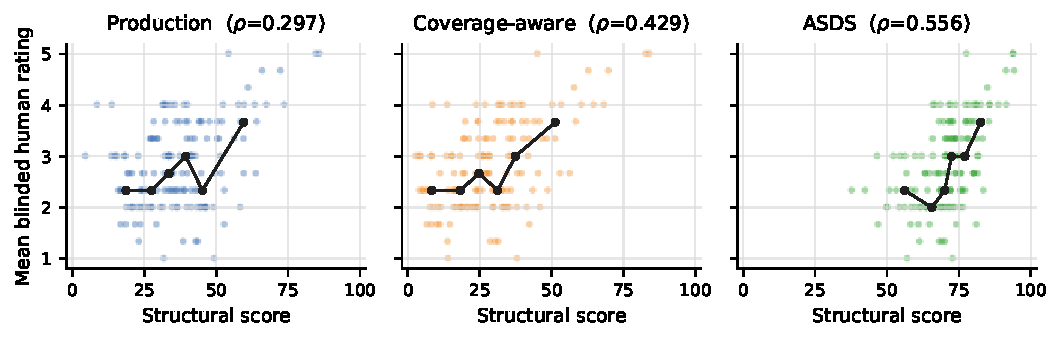
\includegraphics[width=\textwidth]{figures/human_score_association.pdf}
  \caption{Development-stage association between blinded mean structural
  rating and the production, coverage-aware, and ASDS scores for 150 natural
  same-character pairs. Points are individual pairs; lines connect score-bin
  medians only as a descriptive guide. ASDS was designed after these ratings,
  so this figure is not an independent validation.}
  \label{fig:human-score-association}
\end{figure*}

Figure~\ref{fig:human-score-association} visualizes the stronger monotonic
organization of ASDS while preserving the substantial dispersion that
motivates independent confirmation.

\subsection{RQ4: diagnostic feedback}

\begin{table}[t]
\caption{Primary taxonomy of exact-region diagnostic failures.}
\label{tab:feedback-failures}
\centering
\small
\begin{tabular}{lrr}
\toprule
Failure type & Count & Fraction \\
\midrule
multi\_region\_or\_grid\_boundary\_truth & 1922 & 0.539 \\
wrong\_direction\_channel & 876 & 0.246 \\
local\_finding\_absent\_from\_top3 & 718 & 0.201 \\
wrong\_missing\_extra\_type & 38 & 0.011 \\
alignment\_residual\_region\_shift & 11 & 0.003 \\
\bottomrule
\end{tabular}
\end{table}


Table~\ref{tab:feedback-failures} separates the dominant localization failure
types. Required Recall@3 is 0.701, whereas exact grid-region localization is
0.109.
Among exact-region failures, 53.9\% occur because the perturbation truth spans
multiple cells while the metric requires one exact cell, 24.6\% involve an
incorrect direction channel, and 20.1\% contain no local finding in the top
three. Wrong missing/extra type and residual registration shifts are uncommon.
The main limitation is therefore a mixture of localization representation and
direction attribution rather than wording. This motivates a future set- or
pixel-overlap localization metric, not further tuning of feedback rules on the
same cases.
